\documentclass[a4paper, 12pt]{article}
\usepackage{hyperref}
\usepackage{xcolor}
\usepackage{graphicx}
\usepackage{float}
\usepackage[export]{adjustbox}
\usepackage[english]{babel}
\usepackage[T1]{fontenc}
\usepackage{url}
\usepackage{import}
\usepackage{multirow}
\usepackage{color}
\usepackage{fancyhdr}
\usepackage{amssymb}
\usepackage{tabu}
\usepackage{listings}
\usepackage[margin=2.5cm]{geometry}
\usepackage{titling}
\usepackage{listingsutf8}
\usepackage[utf8]{inputenc}
\usepackage{mathtools}
\usepackage[numbered,framed]{matlab-prettifier}
\usepackage{amsmath}
\usepackage{animate}
\usepackage[labelformat=empty]{caption}
\usepackage{subfig}

\let\ph\mlplaceholder
\lstMakeShortInline"

\newcommand{\bnb}{\begin{nobreak}}
\newcommand{\enb}{\end{nobreak}}

\lstset{
	style              = Matlab-editor,
	basicstyle         = \mlttfamily,
	escapechar         = ",
	mlshowsectionrules = true,
}

\title{\vspace{2cm}Elaborato di\\ \textbf{Calcolo Numerico}\\ Anno Accademico 2017/2018\vspace{1cm}}



\begin{document}
	
	\pagenumbering{Roman}
	\lstset{inputencoding=latin1}
	
	\maketitle
	
	\begin{center}
		\today{}
	\end{center}
	
	\newpage
	
	\newpage
	
	\tableofcontents
	\newpage
	
	\pagenumbering{arabic}
	
	\vspace{0.8cm}
\section{\textbf{Capitolo 4}}
\subsection{}
\begin{center}
	\large\noindent\fbox{
		\parbox{\textwidth}{
			Scrivere una function Matlab che implementi il calcolo del polinomio interpolante di grado \textit{n} in forma di Lagrange. \\La forma della function deve essere del tipo: \lstinline[language=Matlab]{y = lagrange( xi, fi, x)}
		}
}\end{center}

\noindent Il seguente codice Matlab implementa la function richiesta.

\lstinputlisting[language=Matlab]{Codici/Cap4/lagrange.m}
\newpage
\subsection{}
\begin{center}
\large\noindent\fbox{
	\parbox{\textwidth}{
	Scrivere una function Matlab che implementi il calcolo del polinomio interpolante di grado \textit{n} in forma di Newton. \\La forma della function deve essere del tipo: \lstinline[language=Matlab]{y = newton( xi, fi, x)}
	}
}\end{center}

\noindent Il seguente codice Matlab implementa la function richiesta.

\lstinputlisting[language=Matlab]{Codici/Cap4/newton.m}
\newpage
\subsection{}
\begin{center}
\large\noindent\fbox{
	\parbox{\textwidth}{
	Scrivere una function Matlab che implementi il calcolo del polinomio interpolante di Hermite. \\La forma della function deve essere del tipo: \lstinline[language=Matlab]{y = hermite( xi, fi, f1i, x)}
	}
}\end{center}

\noindent Il seguente codice Matlab implementa la function richiesta.

\lstinputlisting[language=Matlab]{Codici/Cap4/hermite.m}
\newpage
\subsection{}
\begin{center}
\large\noindent\fbox{
	\parbox{\textwidth}{
	Utilizzare le functions degli esercizi precedenti per disegnare l'approssimazione della funzione \(\sin(x)\) nell'intervallo \([0, 2\pi]\), utilizzando le ascisse di interpolazione \(x_i=i\pi\), \(i= 0,1,2\).
	}
}\end{center}

\noindent Il seguente codice Matlab contiene le chiamate alle funzioni degli esercizi precedenti: \\ \textit{y = newton(xi, fi, x)}; \\ \textit{y = lagrange(xi, fi, x)}; \\ \textit{y = hermite(xi, fi, f1i, x)}; \\ 
calcolate fornendo in input le ascisse \(0, \pi, 2\pi \) e la loro immagine attraverso \(f\)=\(\sin(x)\). Nel caso di Hermite anche la loro immagine attraverso \(f'\)=\(\cos(x)\).

\lstinputlisting[language=Matlab]{Codici/Cap4/Es4_Cap4.m}

\pagebreak
\noindent Nella figura sottostante \'e riportata l'approssimazione della funzione \(\sin(x)\) tramite l'utilizzo delle funzioni di interpolazione:\\

\begin{figure}[H]
	\centering
	\label{Cap4_Es_4}
	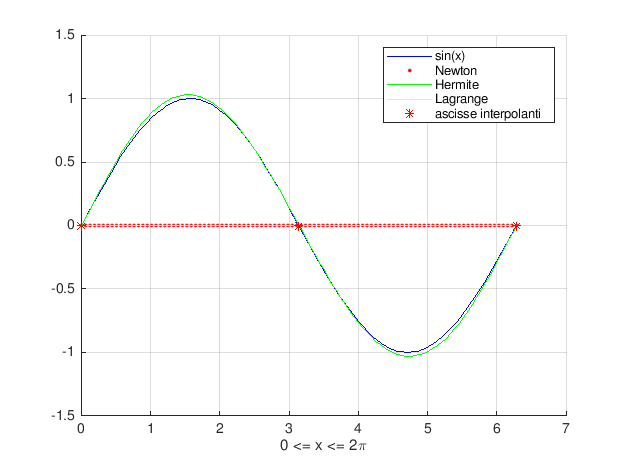
\includegraphics[width=\textwidth,height=\textheight,keepaspectratio]{Codici/Cap4/es4_cap4.png}
\end{figure}

\noindent Essendo \(f_i=0\) per tutte le ascisse \(x_i\), sia il polinomio interpolante di Lagrange, che quello di Newton in realt\'a sono la retta \(y=0\). \\ \\
\newpage
\subsection{}
\begin{center}
\large\noindent\fbox{
	\parbox{\textwidth}{
	Scrivere una function Matlab che implementi la \textit{spline} cubica interpolante (naturale o \textit{not-a-knot}, come specificato in ingresso) delle coppie di dati assegnate. La forma della function deve essere del tipo: \lstinline[language=Matlab]{y = spline3( xi, fi, x, tipo)}
	}
}\end{center}

\noindent I seguenti codici Matlab, contengono la soluzione al problema dato:

\lstinputlisting[language=Matlab]{Codici/Cap4/spline3.m}

\pagebreak

\lstinputlisting[language=Matlab]{Codici/Cap4/diffDivise.m}

\vspace*{0.5cm}

\lstinputlisting[language=Matlab]{Codici/Cap4/solveSplineNat.m}

\pagebreak

\lstinputlisting[language=Matlab]{Codici/Cap4/solveSplineNaK.m}

\pagebreak

\lstinputlisting[language=Matlab]{Codici/Cap4/createSpline.m}

\vspace*{0.5cm}

\lstinputlisting[language=Matlab]{Codici/Cap4/evaluateSpline.m}
\newpage
\subsection{}
\begin{center}
\large\noindent\fbox{
	\parbox{\textwidth}{
	Scrivere una function Matlab che implementi il calcolo delle ascisse di Chebyshev per il polinomio interpolante di grado \textit{n}, su un generico intervallo \([a, b]\). \\ \\La function deve essere del tipo: \lstinline[language=Matlab]{ xi = ceby( n, a, b )}
	}
}\end{center}

\noindent Il seguente codice Matlab implementa la function richiesta.

\lstinputlisting[language=Matlab]{Codici/Cap4/ceby.m}
\subsection{}
\begin{center}
\large\noindent\fbox{
	\parbox{\textwidth}{
	Utilizzare le function degli Esercizi 4.1 e 4.6 per graficare l'approssimazione della funzione di Runge sull'intervallo \([-6, 6]\), per \(n = 2, 4, 6, \ldots, 40\). Stimare numericamente l'errore commesso in funzione del grado \textit{n} del polinomio interpolante.
	}
}\end{center}

\noindent Il seguente codice Matlab implementa la soluzione al problema dato: 
\lstinputlisting[language=Matlab]{Codici/Cap4/Esercizio7_Cap4.m}
\vspace*{1cm}
\noindent Il grafico seguente mostra i polinomi interpolanti di grado \textit{n}, calcolati utilizzando come punti di interpolazione quelli corrispondenti alle \textit{n} ascisse di Chebyshev. Si ricorda la funzione di Runge scritta come:  \(f(x) = \frac{1}{1+25x^2}\). \\

\hspace{3.5cm}

\begin{figure}[H]
	\centering
    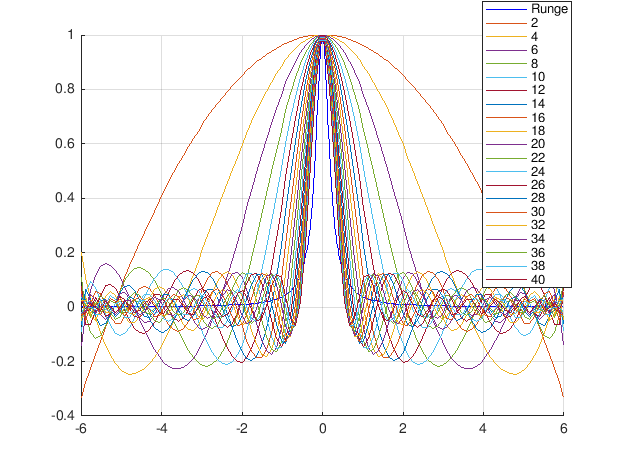
\includegraphics[width=\textwidth,height=\textheight,keepaspectratio]{Codici/Cap4/es7_cap4.png}
\end{figure}

\pagebreak
\noindent Abbiamo quindi calcolato l'errore al variare di $n$ (con $f$ = funzione di Runge e $p_n(x)$ = il suo polinomio interpolante di grado $n$) come segue:

$$
||err|| \approx ||f(x) - p_n(x)||_{\inf}
$$

\noindent Nella seguente tabella si riportano gli errori calcolati: 

\begin{center}
	\begin{tabular}{|c|c|}
		\hline
		$n$ & $\|err\|$ \\
		\hline
		$2$  & $0.9244$ \\
		$4$  & $0.8717$ \\
		$6$  & $0.8217$ \\
		$8$  & $0.7757$ \\
		$10$ & $0.7262$ \\
		$12$ & $0.6866$ \\
		$14$ & $0.6464$ \\
		$16$ & $0.6025$ \\
		$18$ & $0.5568$ \\
		$20$ & $0.5291$ \\
		$22$ & $0.5000$ \\
		$24$ & $0.4696$ \\
		$26$ & $0.4384$ \\
		$28$ & $0.4067$ \\
		$30$ & $0.3747$ \\
		$32$ & $0.3427$ \\
		$34$ & $0.3110$ \\
		$36$ & $0.2855$ \\
		$38$ & $0.2713$ \\
		$40$ & $0.2570$ \\
		\hline
	\end{tabular}
\end{center} 


\noindent Grazie alla scelta delle ascisse di Chebyshev come punti di interpolazione, l'errore diminuisce all'aumentare di \(n\).
\newpage
\subsection{}
\begin{center}
\large\noindent\fbox{
	\parbox{\textwidth}{
	Relativamente al precedente esercizio, stimare numericamente la crescita della costante di Lebesgue.
	}
}\end{center}

\noindent I seguenti codici Matlab contengono il calcolo della costante di Lebesgue in funzione di $n$. La costante di Lebesgue è definita come segue:

\[
\Lambda_n = ||\lambda_n|| \quad con \ \lambda_n(x) = \sum_{i=0}^{n} |L_{(i,n)}(x)|
\]

\lstinputlisting[language=Matlab]{Codici/Cap4/Esercizio8_Cap4.m}

\lstinputlisting[language=Matlab]{Codici/Cap4/computeLeb.m}
\pagebreak

\noindent Nella seguente tabella viene mostrata come varia la costante di Lebesgue in funzione di $n$. Come si può notare, grazie alle ascisse di Chebyshev, si ha una crescita logaritmica della costante al variare del grado n del polinomio: 

\begin{center}
	\begin{tabular}{|c|c|}
		\hline
		$n$ & $lebesgue$ \\
		\hline
		$2$  & $1.2500$ \\ 
		$4$  & $1.5702$ \\ 
		$6$  & $1.7825$ \\ 
		$8$  & $1.9416$ \\ 
		$10$ & $2.0687$ \\ 
		$12$ & $2.1747$ \\ 
		$14$ & $2.2655$ \\ 
		$16$ & $2.3450$ \\ 
		$18$ & $2.4156$ \\ 
		$20$ & $2.4792$ \\ 
		$22$ & $2.5370$ \\ 
		$24$ & $2.5900$ \\ 
		$26$ & $2.6386$ \\ 
		$28$ & $2.6843$ \\ 
		$30$ & $2.7266$ \\ 
		$32$ & $2.7662$ \\ 
		$34$ & $2.8036$ \\ 
		$36$ & $2.8391$ \\ 
		$38$ & $2.8718$ \\ 
		$40$ & $2.9022$ \\ 
		\hline
	\end{tabular}
\end{center} 


\newpage
\subsection{}
\begin{center}
\large\noindent\fbox{
	\parbox{\textwidth}{
	Utilizzare la function dell'Esercizio 4.1 per approssimare la funzione di Runge sull'intervallo \([-6,6]\), su una partizione uniforme di \(n+1\) ascisse per \(n = 2,4,6, \ldots,40\). Stimare le corrispondenti costanti di Lebesgue.
	}
}\end{center}

\noindent Il seguente codice Matlab contiene la soluzione al problema dato:

\lstinputlisting[language=Matlab]{Codici/Cap4/Esercizio9_Cap4.m}

\pagebreak
\noindent Di seguito i grafici mostrano i polinomi interpolanti di Lagrange al variare del grado  $N$ con \(N = 2,4,6, \ldots,40\).

\begin{figure}[H]
	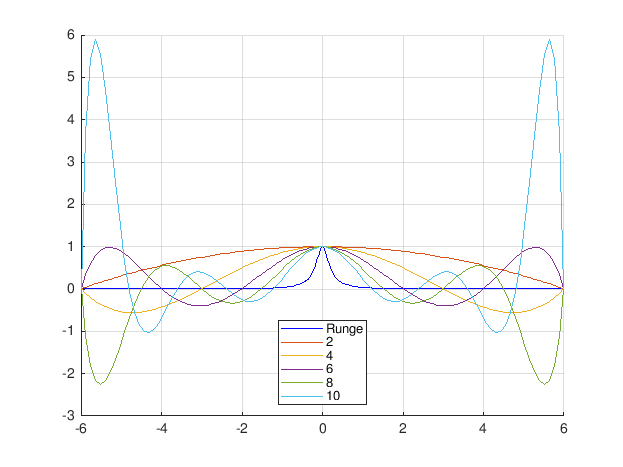
\includegraphics[height=0.6\textwidth,width=\textwidth]{Codici/Cap4/es9(n10)}
\end{figure}

\begin{figure}[H]
	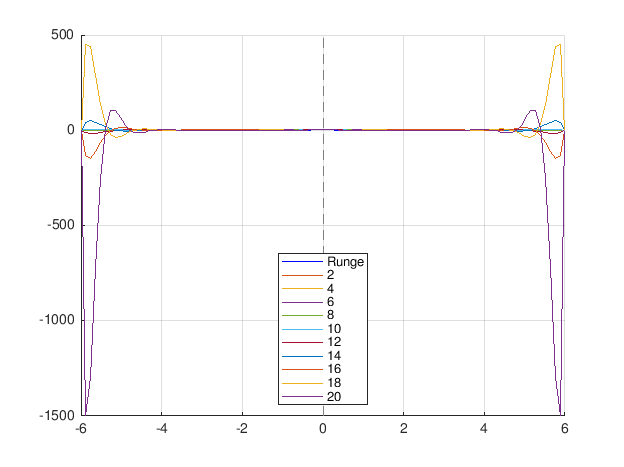
\includegraphics[width=\textwidth]{Codici/Cap4/es9(n20)}
\end{figure}

\begin{figure}[H]
	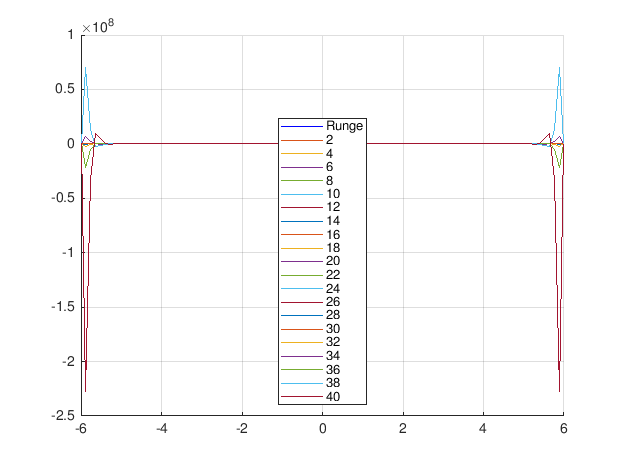
\includegraphics[height=0.6\textwidth,width=\textwidth]{Codici/Cap4/es9(n40)}
\end{figure}

Nella tabella è riportato come varia la \textit{costante di Lebesgue}, al variare del grado \textit{n} del polinomio interpolante. Come si può vedere, all'aumentare di \textit{n} l'errore aumenta a causa della scelta delle ascisse equispaziate.

\begin{center}
	\begin{tabular}{|c|c|}
		\hline
		$n$ & $lebesgue$ \\
		\hline
		$2$  & $0.9342$ \\ 
		$4$  & $0.8566$ \\ 
		$6$  & $0.9846$ \\ 
		$8$  & $2.2590$ \\ 
		$10$ & $5.8960$ \\ 
		$12$ & $16.3788$ \\ 
		$14$ & $49.2750$ \\ 
		$16$ & $147.6550$ \\ 
		$18$ & $450.3933$ \\ 
		$20$ & $1.5025e+03$ \\ 
		$22$ & $5.0066e+03$ \\ 
		$24$ & $1.6654e+04$ \\ 
		$26$ & $5.5282e+04$ \\ 
		$28$ & $1.8307e+05$ \\ 
		$30$ & $6.0468e+05$ \\ 
		$32$ & $1.9918e+06$ \\ 
		$34$ & $6.5422e+06$ \\ 
		$36$ & $2.1426e+07$ \\ 
		$38$ & $6.9960e+07$ \\ 
		$40$ & $2.2774e+08$ \\ 
		\hline
	\end{tabular}
\end{center}
\newpage
\subsection{}
\begin{center}
\large\noindent\fbox{
	\parbox{\textwidth}{
	Stimare, nel senso dei minimi quadrati, posizione, velocit\'a iniziale ed accelerazione relative ad un moto rettilineo uniformemente accelerato per cui sono note le seguenti misurazioni dele coppie \((tempo, spazio)\):\\
	\((1, 2.9) \quad (1, 3.1)\quad (2, 6.9) \quad (2, 7.1) \quad (3, 12.9) \quad (3, 13.1) \quad (4, 20.9) \quad (4, 21.1) \quad (5, 30.9) \quad (5, 31.1)\)
	}
}\end{center}

\noindent La legge che descrive il fenomeno del moto rettilineo uniformemente accelerato si pu\'o scrivere in forma polinomiale come segue:

\[
y =  s(t) = x_0 + v_0t + a_0t^2 \quad \quad \text{con } a_0 = \frac{1}{2}a
\]

\noindent Il cui grado è n = 2. Il sistema ha soluzione se si ha almeno n+1 punti distinti.
In questo caso il problema \'e ben posto poich\'e i punti distinti sono 5>3.

\noindent Si vuole quindi stimare nel senso dei minimi quadrati: posizione, velocità iniziale, ed accelerazione, che equivale alla risoluzione del sistema lineare sovradeterminato:
\[
V\underline{a}=\underline{y}
\]

\noindent con $V$ matrice di tipo \textit{Vandermonde} (la trasposta di una matrice di tipo Vandermonde), \underline{a} vettore delle incognite e  \underline{y} il vettore dei valori misurati. \\
\noindent Tale sistema si risolve mediante fattorizzazione \textit{QR}. La matrice $V$ è scritta come segue: 

\[
V=\begin{bmatrix}
x_0^0 & x_0^1 & \cdots & x_0^m \\
x_1^0 & x_1^1 & \cdots & x_1^m \\
\vdots & \vdots & & \vdots \\
x_n^0 & x_n^1 & \cdots & x_n^m \\		
\end{bmatrix}
\]
\vspace*{0.5cm}

\lstinputlisting[language=Matlab]{Codici/Cap4/SoluzioneEs10_Cap4.m}

\noindent Le soluzioni, calcolate, al problema dato sono :
\begin{center}
	$x_0 = 1$, $v_0 = 1$, $a_0 = 1$ 
\end{center}

	\newpage
	\vspace{0.8cm}
\section{\textbf{Capitolo}}
\subsection{}
\begin{center}
\large\noindent\fbox{
	\parbox{\textwidth}{
	  Scrivere una function Matlab che generi la matrice \textit{sparsa} $n \times n$, con $n > 10$

$$
A_n = \begin{pmatrix} a_{11} & \ldots & a_{1n} \\ \vdots & & \vdots \\ a_{n1} & \ldots & a_{nn}\end{pmatrix} \text {, con } a_{ij} =  \begin{cases} 4 \text{ se } i = j \\ -1 \text{ se } i = j \pm 1 \\ -1 \text{ se } i = j \pm 10\end{cases}
$$

Utilizzare,a questo fine, la function Matlab spdiags.
}
}\end{center}

\noindent Il seguente codice Matlab risolve il problema dato utilizzando la funzione \lstinline[language=Matlab]{spdiags}:

\lstinputlisting[language=Matlab]{Codici/Cap6/createSparseMatrix.m}
\newpage
\subsection{}
\begin{center}
\large\noindent\fbox{
	\parbox{\textwidth}{
    Utilizzare il metodo delle potenze per calcolarne l'autovalore dominante della matrice $A_n$ del precedente esercizio, con una approssimazione $tol=10^{-5}$, partendo da un vettore con elementi costanti. Riempire, quindi, la seguente tabella: \\ \begin{center}
  \begin{tabular}{ | l | c | r |}
    \hline
    $n$ & \textit{numero iterazioni effettuate} & \textit{stima autovalore} \\ \hline
    100 &  &  \\ 
    200 &  &  \\ 
    \vdots &  &  \\  
	1000 &  &  \\
    \hline
  \end{tabular}
\end{center}
}
}\end{center}
\noindent Di seguito sono riportati i codici implementati. La funzione \textit{potenze} calcola sia l'autovalore dominante della matrice \textit{A} , sia il numero di iterazioni, \textit{numIt }, impiegate.
\vspace{0.5cm}

\lstinputlisting[language=Matlab]{Codici/Cap6/SoluzioneEs2_Cap6.m}
\lstinputlisting[language=Matlab]{Codici/Cap6/potenze.m}

\noindent Nella seguente tabella \'e possibile visualizzare i risultati ottenuti: 

\begin{center}
	\begin{tabular}{ | l | c | c |}
		\hline
		$n$ & \textit{numero iterazioni effettuate} & \textit{stima autovalore} \\ \hline
		$100$ & $167$ & $7.8224$ \\
		$200$ & $420$ & $7.8803$ \\
		$300$ & $638$ & $7.8916$ \\
		$400$ & $721$ & $7.8949$ \\
		$500$ & $743$ & $7.8964$ \\
		$600$ & $824$ & $7.8974$ \\
		$700$ & $893$ & $7.8976$ \\
		$800$ & $868$ & $7.8967$ \\
		$900$ & $795$ & $7.8957$ \\
		$1000$ & $775$ & $7.8954$ \\
		\hline
	\end{tabular}
\end{center}
\newpage
\subsection{}
\begin{center}
\large\noindent\fbox{
	\parbox{\textwidth}{
	  Utilizzare il metodo di Jacobi per risolvere il sistema lineare
	  $$
	  A_n \textbf{x} = \begin{pmatrix} 1 \\ \vdots \\ 1 \end{pmatrix}
	  $$

	  dove $A_n$ è la matrice definita nell'Esercizio 6.1, con tolleranza $tol=10^{-5}$, e partendo dal vettore nullo. Graficare il numero di iterazioni necessarie, rispetto alla dimensione $n$ del problema, con $n$ che varia da 100 a 1000 (con passo 20).
}
}\end{center}

\noindent Di seguito si riportano i codici Matlab utilizzati. La funzione di \textit{Jacobi} oltre ad effettuare il calcolo del vettore delle incognite della matrice $A$, restituisce anche il numero di iterazioni \textit{numIt} impiegate e la norma infinito del residuo, al passo i-simo.

\lstinputlisting[language=Matlab]{Codici/Cap6/SoluzioneEs3_Cap6.m}
\vspace*{0.5cm}
\lstinputlisting[language=Matlab]{Codici/Cap6/jacobi.m}
\vspace*{1cm}
\noindent Graficamente si pu\'o osservare il seguente risultato, al variare di \textit{n}: 

\begin{figure}[H]
	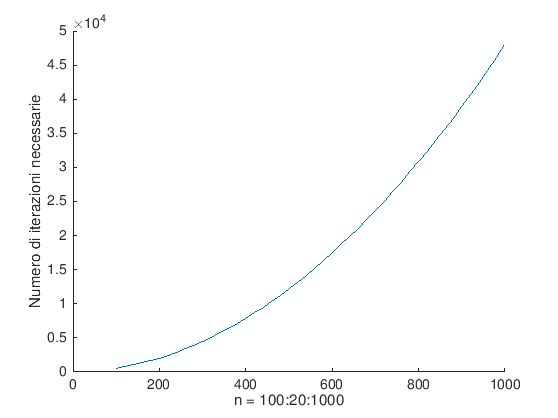
\includegraphics[width=\textwidth]{Codici/Cap6/es3_cap6}
\end{figure}
\newpage
\subsection{}
\begin{center}
\large\noindent\fbox{
	\parbox{\textwidth}{
	 Ripetere una procedura analoga a quella del precedente esercizio utilizzando il metodo di Gauss-Seidel.
}
}\end{center}

\noindent Il codice Matlab utilizzato per realizzare il grafico \'e il seguente:

\lstinputlisting[language=Matlab]{Codici/Cap6/Soluzione4_Cap6.m}

\vspace*{0.5cm}

\lstinputlisting[language=Matlab]{Codici/Cap6/gaussSeidel.m}

\vspace*{0.5cm}

\lstinputlisting[language=Matlab]{Codici/Cap6/trisolveInfGaussSeidel.m}

\noindent Grafico risultante: 

\begin{figure}[H]
	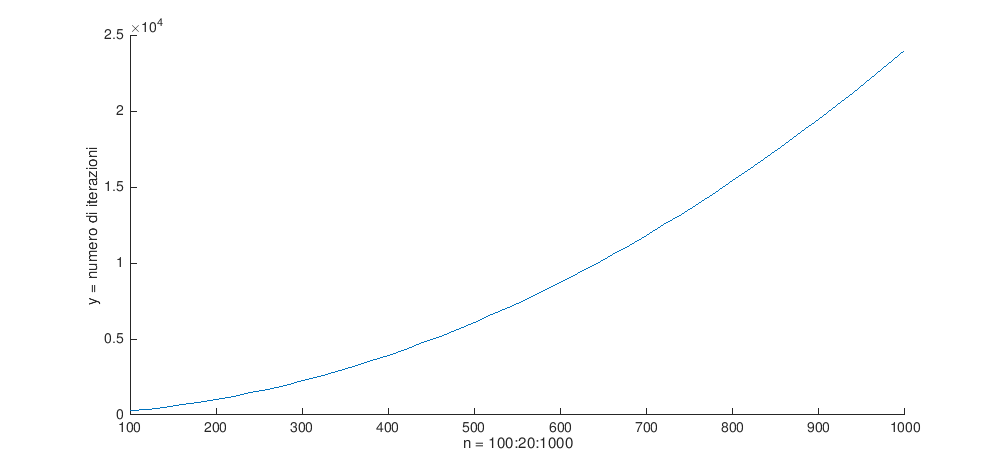
\includegraphics[width=\textwidth]{Codici/Cap6/es4cap6}
\end{figure}

\newpage
\subsection{}
\begin{center}
\large\noindent\fbox{
	\parbox{\textwidth}{
Con riferimento al sistema lineare dell' Esercizio 6.3, con $n=1000$, graficare la norma dei residui, rispetto all'indice di iterazione, generati dai metodi di Jacobi e Gauss-Seidel. Utilizzare il formato \textit{semilogy} per realizzare il grafico, corredandolo di opportune $label$.
} }
\end{center}

\noindent Il seguente codice Matlab \'e stato utilizzato per la risoluzione del problema:

\lstinputlisting[language=Matlab]{Codici/Cap6/SoluzioneEs5_Cap6.m}

\vspace*{1cm}

\noindent Il grafico seguente mostra la norma dei residui, rispetto all'indice di iterazione generati dai metodi di Jacobi (in azzurro) e Gauss-Seidel (in rosso):


\begin{figure}[H]
	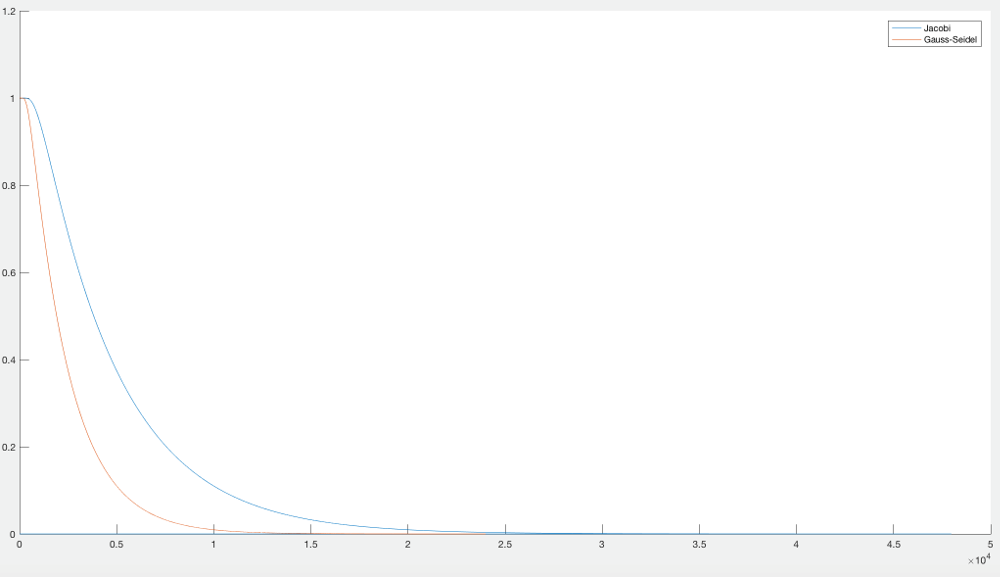
\includegraphics[width=\textwidth]{Codici/Cap6/Es5_Cap61}
\end{figure}
\newpage
    \newpage

	
\end{document}